\part{Mitigation}
\section{Mitigation}

\begin{frame}
	\partpage
\end{frame}

%%%%%%%%%%%%%%%%%%%%%%%%%%%%%%%%%%%%%%%%%%%%%%%%%%%%%%%%%%%%%%%%%%%%%%%%%%%%%%%
\begin{frame}
	\frametitle{Preventing compromise of SSH servers}
	
	
	Very difficult to determine the infection vector used to install these OpenSSH backdoors.
	
	\medskip
	
	In the operation Windigo two different vector was used: 
	
	\smallskip
	
	An attack of the website \textbf{\textit{kernel.org}} (the official repository of the linux kernel source code) to inject malicious code.
	
	\smallskip
	
	An attack to \textbf{\textit{cpanel.net}}, the most famous software to manage websites and hosting.

  \medskip
  
  Obvious but important recommendation is to install software only from trusted sources, e.g. checks sources in \textsc{/etc/apt/sources.list} for debian-derived linux distribution or install only trusted package from the AUR (Arch User Repository) for ArchLinux distribution. 
  	
\end{frame}
%%%%%%%%%%%%%%%%%%%%%%%%%%%%%%%%%%%%%%%%%%%%%%%%%%%%%%%%%%%%%%%%%%%%%%%%%%%%%%%


%%%%%%%%%%%%%%%%%%%%%%%%%%%%%%%%%%%%%%%%%%%%%%%%%%%%%%%%%%%%%%%%%%%%%%%%%%%%%%%
\begin{frame}
	\frametitle{Correct OpenSSH configuration}
	
	It is possible that some attackers could be using \textbf{brute-force} to gain access through SSH password authentication.
	
	\medskip
	
	Good practice is to have long and complex passwords in order to prevent a successful brute-force.
	A better solution is to \textbf{disable password authentication} and use only a key-based authentication. 

  \smallskip
  	
	Set \textsc{PasswordAuthentication no} in \textsc{/etc/ssh/sshd\_config}
	
	\medskip

  If password	login is the only choose setup a limit to failed attempt.
  
	\medskip
	
	Another good practice (almost standard today) is to \textbf{disable remote root login}, in order to prevent login without a named user account. 
	A user can have administrative privileges but can be easily identifies instead of share root password among admins.

  \smallskip
  	
	Set \textsc{PermitRootLogin no} in \textsc{/etc/ssh/sshd\_config}
	
	\medskip

  The most efficient solution would be to use a \textbf{multi-factor authentication} (such as SMS-based verification, a security token or other). 
  OpenSSH still doesn't support this kind of authentication but it can be achieved through an external extension like \textit{google-authenticator-libpam}. 	
  
\end{frame}
%%%%%%%%%%%%%%%%%%%%%%%%%%%%%%%%%%%%%%%%%%%%%%%%%%%%%%%%%%%%%%%%%%%%%%%%%%%%%%%


%%%%%%%%%%%%%%%%%%%%%%%%%%%%%%%%%%%%%%%%%%%%%%%%%%%%%%%%%%%%%%%%%%%%%%%%%%%%%%%
\begin{frame}
	\frametitle{Check logs and network traffic}
	
	\textbf{Enable logs} for every critical service.

	\smallskip

  Periodically \textbf{backup logs} in an external server/device.

	\smallskip
	
	Check for suspicious operations in log files on the server.

	\medskip
	
  \begin{center}    
  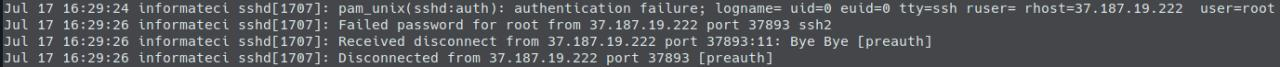
\includegraphics[width=1\textwidth]{images/ssh_log}
  \captionof{figure}{Failed attempt of login in a server}
  \end{center}
  
	\medskip
	
  Setup a firewall and try to monitor all suspicious network traffic (difficult if a lot of traffic is present but can be automatized), block traffic from all unused ports.

\end{frame}
%%%%%%%%%%%%%%%%%%%%%%%%%%%%%%%%%%%%%%%%%%%%%%%%%%%%%%%%%%%%%%%%%%%%%%%%%%%%%%%

%%%%%%%%%%%%%%%%%%%%%%%%%%%%%%%%%%%%%%%%%%%%%%%%%%%%%%%%%%%%%%%%%%%%%%%%%%%%%%%
\begin{frame}
 	\frametitle{Detect compromised SSH tools}
	
	A \textbf{Malware Indicators of Compromise} (IoC) by ESET is publically available \url{https://github.com/eset/malware-ioc}.
	
	The tool can detect malicious OpenSSH files on the system.
	
	\medskip
	
	A good operation is to \textbf{verify integrity} of OpenSSH binaries but ELF file format does not support signatures (unlike PE in Windows or Mach-O on macOS).
	
	\medskip
	
	On a Debian-based distribution commands \textsc{debsums} or \textsc{dpkg -V} can be used to compare installed softwares with a manifest stored on disk, however a local manifest can be easily changed.
	The only solution is to compare the metadata of the \textsc{.deb} package against the one in the \textbf{Debian official repositories}.
	
	\medskip
	
  Backdoor could also be in an \textbf{shared library} instead of client/daemon binary: a modified library can change the behaviour of any application that use it.
  None of the 21 families seems to use this technique, however Ebury backdoor comes with an \textbf{altered version of \textit{libkeyutils.so}}, which is loaded by all OpenSSH process.
  
\end{frame}
%%%%%%%%%%%%%%%%%%%%%%%%%%%%%%%%%%%%%%%%%%%%%%%%%%%%%%%%%%%%%%%%%%%%%%%%%%%%%%%
